\documentclass[25pt, a0paper, landscape]{tikzposter}
\tikzposterlatexaffectionproofoff
\usepackage[utf8]{inputenc}
\usepackage{authblk}
\makeatletter
\renewcommand\maketitle{\AB@maketitle} % revert \maketitle to its old definition
\renewcommand\AB@affilsepx{\quad\protect\Affilfont} % put affiliations into one line
\makeatother
\renewcommand\Affilfont{\Large} % set font for affiliations
\usepackage{amsmath, amsfonts, amssymb}
\usepackage{tikz}
\usepackage{pgfplots}
% align columns of tikzposter; needs two compilations
\usepackage[colalign]{column_aligned}

% tikzposter meta settings
\usetheme{Default}
\usetitlestyle{Default}
\useblockstyle{Default}

%%%%%%%%%%% redefine title matter to include one logo on each side of the title; adjust with \LogoSep
\makeatletter
\newcommand\insertlogoi[2][]{\def\@insertlogoi{\includegraphics[#1]{#2}}}
\newcommand\insertlogoii[2][]{\def\@insertlogoii{\includegraphics[#1]{#2}}}
\newlength\LogoSep
\setlength\LogoSep{-70pt}

\renewcommand\maketitle[1][]{  % #1 keys
    \normalsize
    \setkeys{title}{#1}
    % Title dummy to get title height
    \node[inner sep=\TP@titleinnersep, line width=\TP@titlelinewidth, anchor=north, minimum width=\TP@visibletextwidth-2\TP@titleinnersep]
    (TP@title) at ($(0, 0.5\textheight-\TP@titletotopverticalspace)$) {\parbox{\TP@titlewidth-2\TP@titleinnersep}{\TP@maketitle}};
    \draw let \p1 = ($(TP@title.north)-(TP@title.south)$) in node {
        \setlength{\TP@titleheight}{\y1}
        \setlength{\titleheight}{\y1}
        \global\TP@titleheight=\TP@titleheight
        \global\titleheight=\titleheight
    };

    % Compute title position
    \setlength{\titleposleft}{-0.5\titlewidth}
    \setlength{\titleposright}{\titleposleft+\titlewidth}
    \setlength{\titlepostop}{0.5\textheight-\TP@titletotopverticalspace}
    \setlength{\titleposbottom}{\titlepostop-\titleheight}

    % Title style (background)
    \TP@titlestyle

    % Title node
    \node[inner sep=\TP@titleinnersep, line width=\TP@titlelinewidth, anchor=north, minimum width=\TP@visibletextwidth-2\TP@titleinnersep]
    at (0,0.5\textheight-\TP@titletotopverticalspace)
    (title)
    {\parbox{\TP@titlewidth-2\TP@titleinnersep}{\TP@maketitle}};

    \node[inner sep=0pt,anchor=west] 
    at ([xshift=-\LogoSep]title.west)
    {\@insertlogoi};

    \node[inner sep=0pt,anchor=east] 
    at ([xshift=\LogoSep]title.east)
    {\@insertlogoii};

    % Settings for blocks
    \normalsize
    \setlength{\TP@blocktop}{\titleposbottom-\TP@titletoblockverticalspace}
}
\makeatother
%%%%%%%%%%%%%%%%%%%%%%%%%%%%%%%%%%%%%


% color handling
\definecolor{TumBlue}{cmyk}{1,0.43,0,0}
\colorlet{blocktitlebgcolor}{TumBlue}
\colorlet{backgroundcolor}{white}

% title matter
\title{DL4CV Project}

\author[1]{Strobel Maximilian}
\author[1]{Werhahn Maximilian}
\author[1]{Kiener Martin}
\author[1]{Seferis Emmanouil}

\affil[1]{Technical University of Munich}

\insertlogoi[width=15cm]{tum_logo}
\insertlogoii[width=15cm]{tum_logo}

% main document
\begin{document}

\maketitle

\begin{columns}
    \column{0.3}
    \block{Preprocessing \& Environment}{
    	The environment for the learning agents was OpenAI gym. This toolkit for
    	developing and comparing reinforcement learning agents was used as an interface to Atari 2600
    	games like Breakout or SpaceInvaders, that the agents tried to learn. The interface provides
    	informations about the state of the games as well as the current screen. Due to an internal
    	flickering of the games (e.g. shoots are only on odd frames visible), the current screen is
    	obtained by a maximum operation on two successive frames.
    	Before the screen was feed into the neural network with the screen, it was preprocessed as 	
    	depicted in the graphic below.
		\begin{tikzpicture}
		\node[inner sep=0pt] (preprocessing) at (0,0)
    	{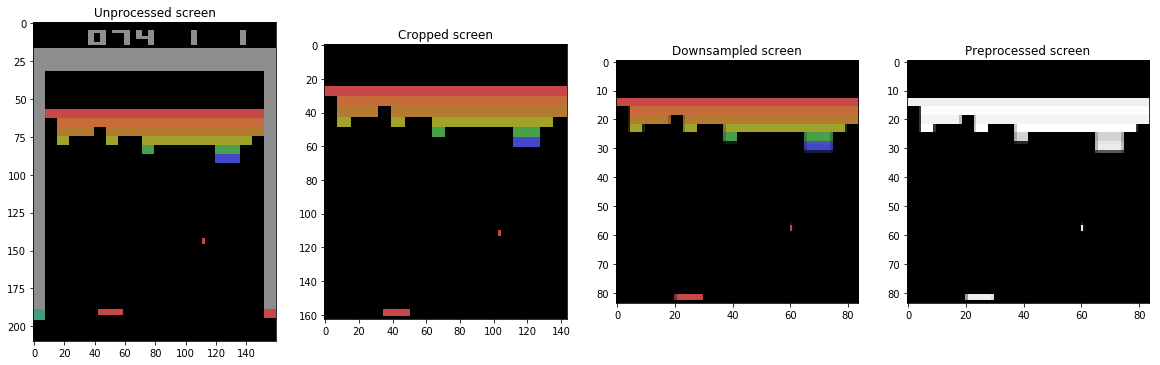
\includegraphics[width=.26\textwidth]{preprocessing_pipeline.png}};
    	\end{tikzpicture}
    	In OpenAI gym there exists a frame skipping technique, that was also modified. Instead of
    	skipping randomly between two and five frames, the frame skipping rate was set to a constant
    	value. During the training the rewards were clamped to -1 and 1 to gain comparability between
    	different games. Additional the lost of one live was punished with an reward of -1, whatever
    	the real reward was.
    }
    \block{First column second block}{Content in your block.}

    \column{0.5}
    \block{First Architecture}{For the first architecture we duplicated the already existing DQN model, removed the output layers of both subnets and added two additional fully connected layers of size 1024 and the maximum of the action spaces of the games to map the input screens of both games to one single action. Each of the two preprocessed frame histories is fed into one of the subnets separately. With this version we already achieved our first goal which is being better than random play.}
    \block{Second column second block}{Content in your block.}
\end{columns}

\end{document}
